In order to test the validity of the Behler-Parrinello method
and AMP, we train and test neural network potentials on the
Lennard-Jones and Stillinger-Weber potentials. These are some of
the simplest realistic potentials, which are widely applied
in the molecular dynamics literature, and fitting to these potentials
will provide much insight into the speed and accuracy of
fitting machine-learned potentials.

\subsection{Lennard-Jones}
The AMP calculator is trained on a Lennard-Jones trajectory
starting in a face-centered-cubic (FCC) crystal
with a lattice spacing of 5.26 Å. We use $2\times2\times2$ unit
cells for a total of $4\cdot2^3 = 64$ atoms, and velocities
are initialized from the Maxwell-Boltzmann distribution
with a temperature of 750 Kelvin.
The atoms are propagated forward using the Verlet integrator
in the microcanonical (NVE) ensemble for $10^4$ steps
with a timestep of $\Delta t = 5$fs, and the trajectory
is written to file every 25 steps.
The potential energy and forces is computed using the Lennard-Jones
potential with the characteristic energy $\epsilon = 1.0318\cdot
10^{-2}$eV and characteristic length $\sigma = 3.405$Å
and a radial cutoff $r_c = 3\sigma$.
\par
Since the Lennard-Jones system is not a very complicated one,
with interactions only reliant on distance we use the AMP
defaults for the symmetry functions.
The AMP defaults for Argon are 4 $G_2$ radial functions
with $\eta = 0.05, 0.23, 1.07, 5.00$ and 4 $G_4$ angular
functions with $\eta = 0.05$, $\gamma = 1.0, -1.0, 1.0, -1.0$
and $\zeta = 1.0, 1.0, 4.0, 4.0$ respectively.
The smooth cutoff function is the cosine function
with a cutoff $r_c = 6.5$Å, which is the default in AMP.
\newline Plot symmetry functions?
\par
The fitting of the neural network requires the selection
of a large number of parameters in order to get an appropriate
convergence. In table \ref{tab:hyperparam} all relevant parameters
are listed.
We have not performed a systematic search over
hyperparameters in this section, so the choice of these is somewhat
arbitrary and based on intuition and rules of thumb.
The network was found to converge on an energy RMSE of approximately
$10^{-3}$eV and a force RMSE of approximately $7.5\cdot10^{-2}$ eV/Å
after a number of trial runs, and these were therefore chosen
as convergence criteria.
The loss function has weightings for both the energy
and the forces, and adding force terms to the loss function
is thought to improve the dynamics of the trained calculator.
However, this requires us to store the force on all atoms
for each image, and may introduce problems with available memory.

\begin{table}[h]
\label{tab:hyperparam}
\caption{Hyperparameters used in fitting.}
\begin{center}
\begin{tabular}{|c c|}
\hline
Hyperparameter & Value \\
\hline \hline
Features & 8 \\
Hidden layers & $(10, 10, 10)$ \\
Activation & Hyperbolic tangent \\
Timesteps & $10^4$ \\
Max epochs & 10000 \\
Optimizer & Adam \\
Initial learning rate & $10^{-3}$ \\
Energy RMSE & $10^{-3}$eV \\
Energy coefficient & 1.0 \\
Force RMSE & $7.5\cdot10^{-2}$eV/Å \\
Force coefficient & 0.04 \\
\hline
\end{tabular}
\end{center}
\end{table}

In figure \ref{fig:convergence} you can see the convergence of the total
loss, and the energy and force RMSEs. The loss has converged
with minor improvements after approximately 200-300 steps,
and then slowly moves toward the criteria until approximately 450 steps.
The loss function is often
quite noisy at the start of the training, but then converges much more
smoothly towards an asymptote. The force RMSE is typically much
larger than the energy RMSE, this is likely because the force RMSE
is averaged over a much larger set of components, which introduces
a lot of noise into the loss.

\begin{figure}[h]
    \centering
    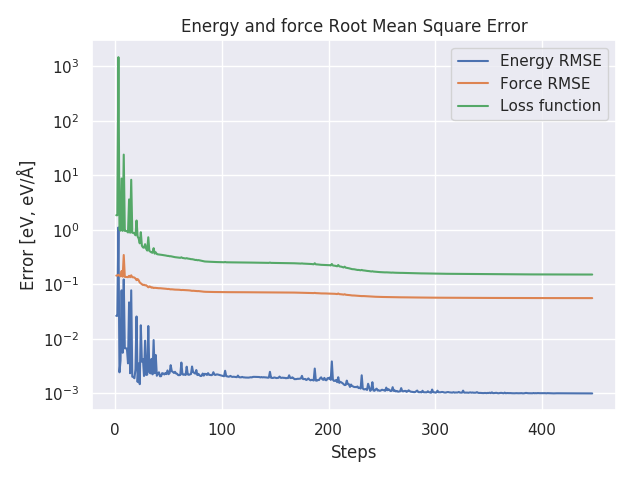
\includegraphics[width=\linewidth]{convergence.png}
    \caption{Convergence}
    \label{fig:convergence}
\end{figure}

After the AMP calculator is trained we use it to generated a 
test trajectory for $10^3$ steps, which is compared to a Lennard-Jones
trajectory of the same size and initial conditions.
In figure \ref{fig:energy} we have plotted a comparison of the
potential energy of the system over time. Typical of any NVE simulation
starting in an equilibrium crystal structure is that some amount of
the initial kinetic energy will be converted to potential energy,
and thereafter the potential energy will stabilize around some value.
We see that the potential energies agree initially, but then the AMP
energy diverges. This is likely a numerical artifact caused by
a poor force fit allowing the atoms to move too closely, and
this will increase the total energy of the system.
This may be improved by further training, a larger dataset or a larger force
coefficient.
\par

\begin{figure}[h]
    \centering
    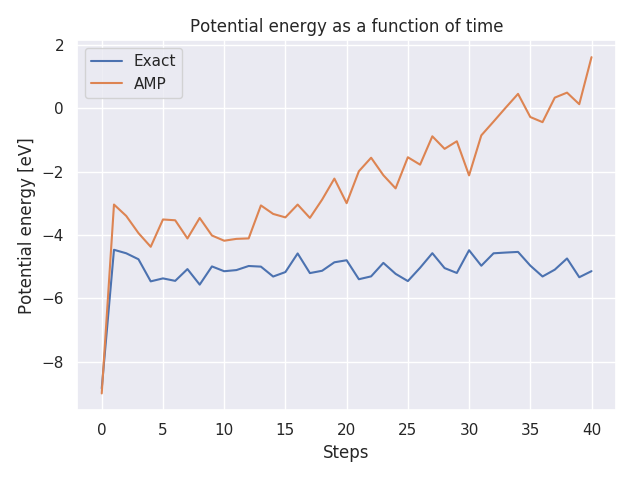
\includegraphics[width=\linewidth]{energy.png}
    \caption{Energy difference}
    \label{fig:energy}
\end{figure}

In figure \ref{fig:rdf} we have plotted the radial distribution function,
which is a good measure of the structural composition of a system.
The radial distribution function measures the density of atoms
at a radial distance from an arbitrarily chosen reference atom.
Any two atoms should not be too close as this implies an enormous
amount of potential energy, and it typically exhibits several
peaks where the atoms prefer to reside. In a homogenous infinite
structure the function approaches unity as the radial distance increases.
If the neural network is to reproduce the correct ensemble averages
we would expect it to exhibit the same structural details.
From the figure we can see the the RDFs mostly exhibit the same
structure and details, which is a good sign. The RDFs do not
overlap completely, which may be improved by further training and 
more data.

\begin{figure}[h]
    \centering
    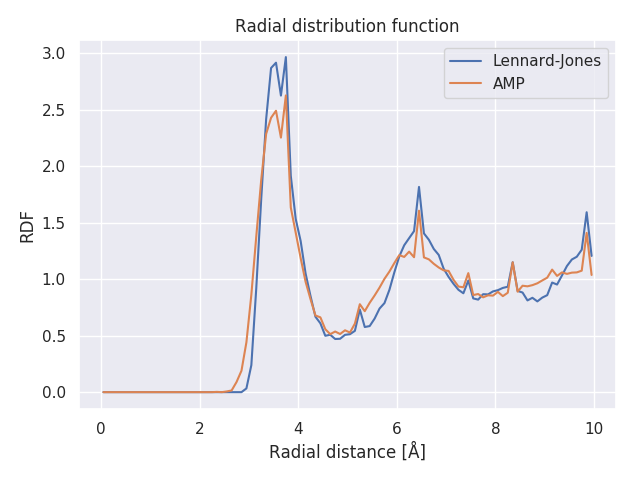
\includegraphics[width=\linewidth]{rdf.png}
    \caption{Radial distribution function}
    \label{fig:rdf}
\end{figure}

In figure \ref{fig:msd} we have plotted the mean squared displacement.
The mean squared displacement measures how an (average) atom
moves with respect to an initial position over time,
and is related to the fraction of the system explored by a random walker.
The mean squared displacement should be linear for a liquid
unaffected by an external force, and can be used to compute
the diffusion constant of the system. If the AMP calculator is accurate
we would expect the diffusion constants to reasonably agree.
We see that the AMP MSD diverges from the Lennard-Jones one
and seems to be increasing sharply over time. This is likely
due to numerical error, with the energy of the system increasing
as the atoms are appearing too close. This should be rectified.

\begin{figure}[h]
    \centering
    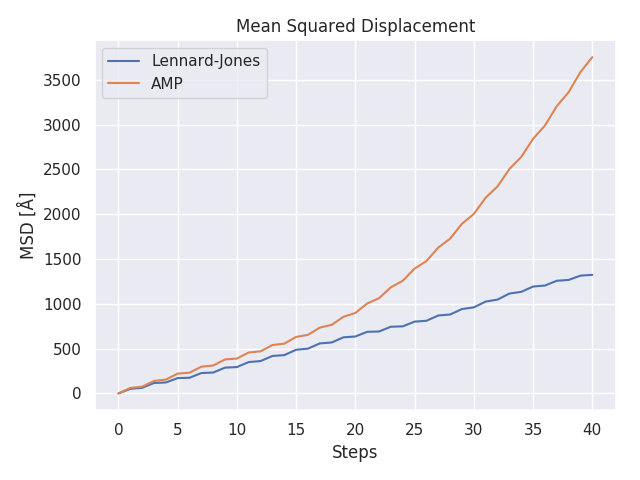
\includegraphics[width=\linewidth]{msd.png}
    \caption{Mean Squared Displacement}
    \label{fig:msd}
\end{figure}

\subsection{Stillinger-Weber}
Text.
